\documentclass{article}
\usepackage{hyperref}
\usepackage{amssymb, mathtools, amsmath}
\usepackage[dvipsnames]{xcolor}
\usepackage{graphicx}
\usepackage{float}
\usepackage{caption}
\usepackage{hyperref}
\hypersetup{
    colorlinks=true,
    linkcolor=blue,
    filecolor=magenta,      
    urlcolor=blue,
}
\usepackage{caption}
\usepackage[margin=0.25in]{geometry}
\usepackage{pgfplots}
\usepgfplotslibrary{external}
\tikzexternalize


\title{ Macroeconomic Theory
        \thanks{Course instructed by Professor Christoph Hedtrich.} \\
        Homework 7: Fiscal Policy
        }

\author{
        Uppsala Masters in Economics 2021-2022
        }

\date{25 November 2021}

% margins
\oddsidemargin 3mm
\evensidemargin 3mm
\topmargin -12mm
\textheight 600pt
\textwidth 420pt

% no indent
\setlength\parindent{0pt}
% \renewcommand{\theenumi}{\thesection(\alph{enumi})}
% \renewcommand\thesubsection{\arabic{subsection}}

% custom commands
\newcommand{\E}[1]{\mathrm{E}\left[#1\right]}
\newcommand{\Et}[1]{\mathrm{E}_t\left[#1\right]}
\newcommand{\cov}[1]{\mathrm{Cov}\left(#1\right)}
\newcommand{\var}[1]{\mathrm{Var}\left(#1\right)}
\renewcommand{\L}{\mathcal{L}}
\newcommand{\?}{\textcolor{red}{(?)}} % question mark

\begin{document}
    
    \maketitle
    
    \section{Debt and Government Spending}
        
        Law of motion for debt:
        \begin{align}
            \dot D(t) = G(t) - T(t) + r(t) D(t)
        \end{align}
        
        Government's budget constraint
        \begin{align}
            \int_{t=0}^\infty e^{-R(t)} G(t) dt 
            \le
            - D(0) + \int_{t=0}^\infty e^{-R(t)} T(t) dt
            \label{eqn:gov-budget}
        \end{align}
        
        
        Consumer's budget constraint,
        \begin{align}
            \int_{t=0}^\infty e^{-R(t)} C(t) dt 
            & \le
            % K(0) + D(0) + 
            % \int_{t=0}^\infty e^{-R(t)} [W(t) - T(t)] dt
            % \\
            % &=
            K(0) + D(0) + 
            \int_{t=0}^\infty e^{-R(t)} W(t) dt
            -
            \int_{t=0}^\infty e^{-R(t)}  T(t) dt
            \\
            &=
            K(0) + 
            \int_{t=0}^\infty e^{-R(t)} W(t) dt
            -
            \int_{t=0}^\infty e^{-R(t)} G(t) dt
            \\
            &=
            K(0) + 
            \int_{t=0}^\infty e^{-R(t)} [W(t) - G(t)] dt
        \end{align}
        
        The \textbf{Ricardian equivalence} makes
        
        But assuming taxes does have distortionary effect. Government's objective is to minimize distortion subject to some compulsory spending.
        \begin{align}
            \min_{T_t}
            \sum_{t=0}^\infty
            \frac{1}{(1+r)^t} \Gamma_t
            &=
            \sum_{t=0}^\infty
            \frac{1}{(1+r)^t}
            Y_t f\left(\frac{T_t}{Y_t}\right)
            \\
            s.t.
            \quad
            D(0) + \sum_{t=0}^\infty \frac{1}{(1+r)^t} G(t)
            &\le
            \sum_{t=0}^\infty \frac{1}{(1+r)^t} T(t)
        \end{align}
        
        where $f'(\cdot) > 0,  f''(\cdot) > 0$. Formulate Lagrangian for minimization:
        \begin{align}
            \mathcal{L}
            &= \sum_{t=0}^\infty
            \frac{1}{(1+r)^t}
            Y_t f\left(\frac{T_t}{Y_t}\right)
            + \lambda \left(
            D(0) + \sum_{t=0}^\infty \frac{1}{(1+r)^t} G(t)
            - \sum_{t=0}^\infty \frac{1}{(1+r)^t} T(t)
            \right)
        \end{align}
        
        Then taking FOC with respect to $T(t)$ at some period $t$, we have:
        \begin{align}
            \frac{\partial \mathcal{L}}{\partial T_t}
            = 0
            &\implies
            \frac{1}{(1+r)^t}
            Y_t f'\left(\frac{T_t}{Y_t}\right) \frac{1}{Y_t} = - \lambda \frac{1}{(1+r)^t}
            \\
            &\implies
            f'\left(\frac{T_t}{Y_t}\right)
            = \lambda
            % \implies
            % \frac{f'\left(\frac{T_t}{Y_t}\right)}{f'\left(\frac{T_{t+1}}{Y_{t+1}}\right)}
            % =\frac{\lambda}{\lambda} = 1
            \\
            &\implies
            f'\left(\frac{T_t}{Y_t}\right)
            = f'\left(\frac{T_{t+1}}{Y_{t+1}}\right)
            \implies
            \frac{T_t}{Y_t} = \frac{T_{t+1}}{Y_{t+1}}
        \end{align}
        Optimal tax rate should be same across period.
    
    \subsection{Question 1: DR 13.1}
    
        \begin{figure}[!ht]
            \centering
            \includegraphics[width=\textwidth]{Homework/HW7/HW7_DR13.1.png}
        \end{figure}
        
        \renewcommand{\theenumi}{(\alph{enumi})}
        \renewcommand{\theenumii}{\roman{enumii}}
        \begin{enumerate}
            \item
            With $\frac{\dot \delta(t)}{D(t)} = g, \; \frac{\dot Y(t)}{Y(t)} = g$, and the fact that $\frac{d}{dt} \ln x(t) = \frac{\dot x(t)}{x(t)}$, we have that
            \begin{align}
                d(t) = \frac{D(t)}{Y(t)}
                \implies
                \ln d(t)
                &= \ln D(t) - \ln Y(t)
                \\
                \implies
                \frac{\dot d(t)}{d(t)}
                &= \frac{\dot D(t)}{D(t)} - \frac{\dot Y(t)}{Y(t)}
                = \frac{\delta(t)}{D(t)} - g
                \\
                &= \frac{aY(t)}{D(t)} - g
                = \frac{a}{d(t)} - g
                \\
                \implies
                \dot d(t)
                &= a - gd(t).
            \end{align}
            
            \item
            We have now that $\delta(t) = a Y(t) + r(t) D(t)$. Then
            \begin{align}
                d(t) = \frac{D(t)}{Y(t)}
                \implies
                \frac{\dot d(t)}{d(t)}
                &= \frac{\dot D(t)}{D(t)} - \frac{\dot Y(t)}{Y(t)}
                = \frac{\delta(t)}{D(t)} - g
                \\
                &= \frac{a Y(t) + r(t) D(t)}{D(t)} - g
                \\
                &= \frac{a}{d(t)} + r(d(t)) - g
                \\
                \implies
                \dot d(t) &= a + (r(d(t)) - g) d(t).
            \end{align}
            
            \begin{figure}[!ht]
                \centering
                \includegraphics[width=0.8\textwidth]{Homework/HW7/HW7_DR13.1-phase_diagram.png}
            \end{figure}
            
        \end{enumerate}
    
    \section{Government Debt Crisis}
    
    \subsection{Question 2: DR 13.16}
        \begin{figure}[h!]
            \centering
            \includegraphics[width=\textwidth]{./HW7-DR13.16.png}
        \end{figure}
        
        Government pays interest factor $R$ on debt $D$, with probability $\pi$ of default, which happens when tax revenue is less than after-interest debt $T < RD$. If default, government pays nothing. In equilibrium, risk-neutral investors imply
        \begin{align}
            0 \pi + R (1-\pi) = \bar R
            \implies
            \pi = \frac{R - \bar R}{R}
        \end{align}
        where $\bar R$ is the risk-free interest rate. Assume government tax revenue $T$ is uniformly distributed. Then probability of default is
        \begin{align}
            \pi = Pr(T < RD)
            = F_{T}(RD)
            = \begin{cases}
                0
                & R < \frac{X - \mu}{D}
                \\
                \frac{RD - (\mu - X)}{2X}
                & R \in \left[
                    \frac{\mu-X}{D}, \frac{\mu+X}{D}
                    \right]
                \\
                1
                & R > \frac{\mu + x}{D}
            \end{cases}
        \end{align}
        
        where $T$ is the tax income, $F(\cdot)$ is the cumulative distribution function. We have equilibria when
        \begin{align}
            \frac{R - \bar R}{R} = Pr(T < RD)
        \end{align}
        
        \pgfplotsset{compat=1.18}
        
        \begin{figure}[H]
            
            \centering
            
            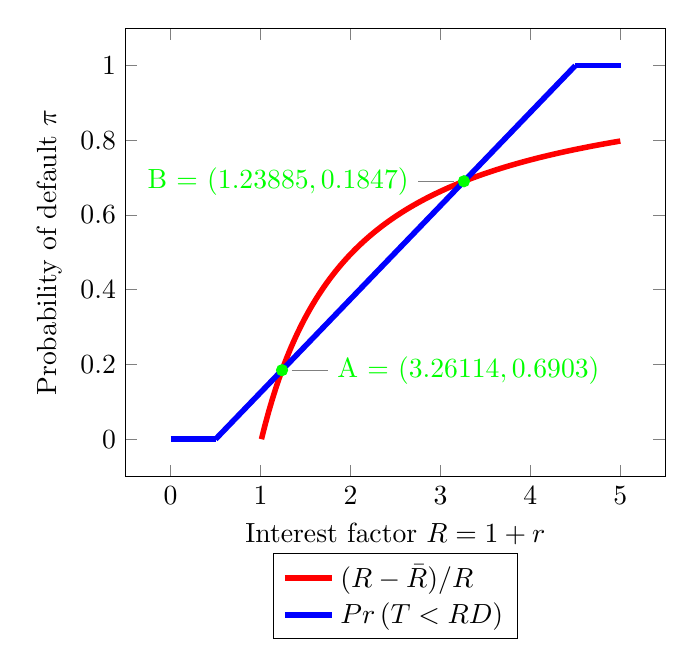
\begin{tikzpicture}
                \begin{axis}[
                    xlabel = {Interest factor \(R = 1+r\)},
                    ylabel = {Probability of default \(\pi\)},
                    legend style={at={(0.5,-0.17)},anchor=north,legend cell align=left}
                    ]
                    
                    % variables
                    \pgfmathsetmacro{\mu}{2.5}
                    \pgfmathsetmacro{\X}{2}
                    
                    \pgfmathsetmacro{\barR}{1.01}
                    \pgfmathsetmacro{\D}{1}
                    
                    \pgfmathsetmacro{\cdfbeg}{(\mu-\X)/\D}
                    \pgfmathsetmacro{\cdfend}{(\mu+\X)/\D}
                    
                    % plot range formatting
                    \pgfmathsetmacro{\xbeg}{0}
                    \pgfmathsetmacro{\xend}{5}
                    \pgfmathsetmacro{\lw}{2}
                    
                    % equilibrium calcuations
                    \pgfmathsetmacro{\RA}{
                    (\mu+\X + ((-\mu-\X)^2-8*\D*\X*\barR)^(1/2)) / (2*\D)
                    }
                    \pgfmathsetmacro{\piA}{(\RA - \barR)/\RA}
                    
                    \pgfmathsetmacro{\RB}{
                    (\mu+\X - ((-\mu-\X)^2-8*\D*\X*\barR)^(1/2)) / (2*\D)
                    }
                    \pgfmathsetmacro{\piB}{(\RB - \barR)/\RB}
                
                    % plot interest-default probability choice
                    \addplot[domain=\barR:\xend, samples=100, color=red, line width=\lw pt] {(x-\barR)/x}; \addlegendentry{\((R - \bar R) / R\)}
            
                    % plot CDF
                    \addplot[domain=\cdfbeg:\cdfend, samples=100, color=blue, line width=\lw pt] {(x*\D-\mu+\X)/(2*\X)}; \addlegendentry{\(Pr\left(T < RD\right)\)}
                    
                    % plot CDF outside of bounds
                    \addplot[domain=\xbeg:\cdfbeg, samples=100, color=blue, line width=\lw pt] {0};
                    \addplot[domain=\cdfend:\xend, samples=100, color=blue, line width=\lw pt] {1};
                    
                    % add equilibrium points
                    \addplot[only marks, color=green, mark=*]
                    coordinates {(\RA, \piA)(\RB, \piB)}
                        node[pos=1, pin=right:{A = \((\RA, \piA)\)}]{}
                        node[pos=0, pin=left:{B = \((\RB, \piB)\)}]{};
                \end{axis}
            \end{tikzpicture}
            \caption{Interest factor-default rate equilibria}
            
        \end{figure}
        
        Then a rise in $\mu$ will shift the $R$ and $\pi$ curve to the right, meaning $R$ will increase for same probability of default. A fall in $X$ shrink the span of the R.
    
    
\end{document}